\section{Visual Object Tracking via Multi-Stream Deep Similarity Learning Networks}

\begin{center}
    \author{
    Kunpeng Li,
    \emph{Student Member, IEEE},
    Yu Kong,
    \emph{Member, IEEE},
    Yunf Fu,
    \emph{Fellow, IEEE}
    }
\end{center}

\begin{center}
    \emph{IEEE TRANSACTIONS ON IMAGE PROCESSING, VOL.29, 2020}
\end{center}

\subsection{INTRODUCTION}
The goal of visual tracking systems is to be able to obtain the position of 
the tracked target even in subsequent frames. The problems to be solved are 
those of occlusion, background clutter, illumination variations, deformation 
etc. The existing state-of-the-art models carry out training online exclusively. 
Some methods, based on pre-trained convolutional networks (CNN), track 
the object based on the background. In these networks, stochastic gradient 
descent is applied in order to update the entire network. However, these 
models appear to be too slow and do not work well in real-time. The following 
paper uses a model that compares similarities and is trained offline in order to 
predict the patch present in the next frame. The method, thanks to the use of 
the relative distance, is robust in the presence of phenomena that introduce 
the so called distractors. The purpose is to be able to compare the patch that 
identifies the target template (the object) with all the possible positions 
of the same region belonging to the next frame. In addition to tracking the 
object, the proposed model is a framework for EMDSLT tracking like the 
one shown in figure \ref{fig:EMDSLT}. Within it, two procedures are considered important: 
updating the model and self-recovery from failures. The network is composed 
of two types of structures, one that is responsible for dast-speed verification 
and production of the tracking results, while the second is responsible for re-verification 
and re-detection of the target object on the patches previously 
generated.
\begin{figure}[h!]
    \centering
    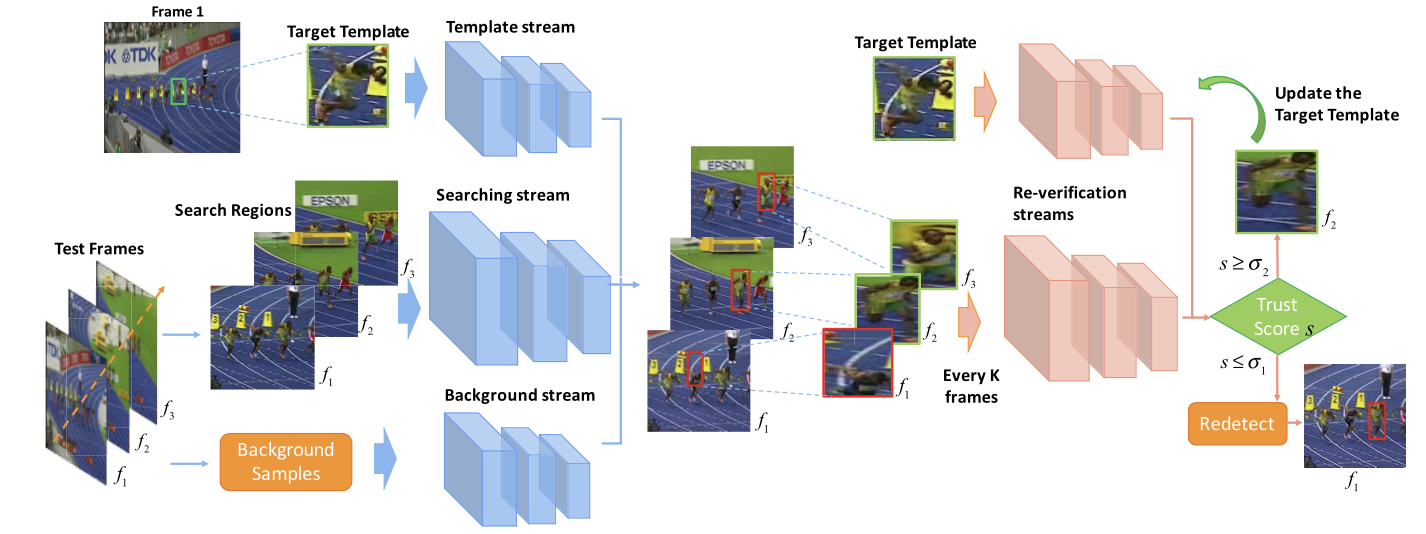
\includegraphics[width = \linewidth]{images/paper8/EMDSLT.png}
    \centering
    \caption{The framework of EMDSLT proposed method.}
    \label{fig:EMDSLT}
\end{figure}.

\subsection{RELATED WORK}
Methods such as generative trackers have been developed for finding positions 
in which to find the best candidate during the tracking process. Good 
results have been achieved by compound trackers \cite{0893551105} \cite{0893551118}. Networks such as 
RNNs \cite{0893551121} can be used to predict possible target positions in each frame. 
However, these types of networks have not yet achieved satisfactory results. 
Some methods instead train a CNN offline while the test is done online. Unfortunately, 
these models are not fast. Other models instead if they fail a first 
time, then they will always fail until the target returns to the search region. 
Methods such as \cite{0893551129} \cite{0893551134} search for the target template in subsequent frames 
in the same position, obtaining better performance than methods based on 
similarity but nevertheless are not robust to distracting elements. The proposed 
method instead takes into account both the background patches and 
the target template patches in order to make comparisons on similarities.

\subsection{METHODS}
\subsubsection{Multi Stream Deep Similarity Learning Networks}
A mulit-stream similarity learning network is used in this paper. In the 
proposed framework there are various data streams (Fig. \ref{fig:EMDSLT}):
\begin{enumerate}
    \item Template Stream: the target template defined in the beginning frame;
    \item Searching Stream: the search region;
    \item Background Stream: background patches that sample around the target 
    in the beginning frame.
\end{enumerate}

\subsubsection{Template-Searching-Background Loss}
Several positive $X^+_i$, negative $X^-_i$ and background $B_{i-1,j}$ patches can be generated in an image. Patches are considered positive if they have a small cosine distance with the target template $T$, on the contrary, patches will be considered negative if they are closer to the background patches within the search region $S_i$. The loss function to be minimized is the following:
\begin{equation}
    L(T,\{X_{i,k}\}^N_{k=1}, \{B_{i-1}\}^M_{j=1}) = \sum_{k=1}^NL(T,X_{i,k}, \{B_{i-1,j}\}^M_{j=1})
\end{equation}
Where $T$ is the target template, $X_{i,k}$ is the $k-th$ candidate patch $X$ of frame $i$, $M$ is the number of background patches and $N$ is the number of candidate patches $X_{i,k}$.